\documentclass[10pt]{article}
\usepackage[margin=1in, paperwidth=8.5in, paperheight=11in]{geometry}
\usepackage{ifpdf,amsmath, amssymb, comment, color, graphicx, stmaryrd,setspace,enumitem,tikz, fancyhdr, wrapfig, textcomp, mathptmx, siunitx}

\setlength{\headheight}{14.5pt}
\newcommand{\Q}{\mathbb{Q}}
\newcommand{\R}{\mathbb{R}}
\newcommand{\Z}{\mathbb{Z}}
\newcommand{\vu}{\mathbf{u}}
\newcommand{\vv}{\mathbf{v}}
\newcommand{\vw}{\mathbf{w}}
\newcommand{\vi}{\mathbf{i}}
\newcommand{\vj}{\mathbf{j}}
\newcommand{\vk}{\mathbf{k}}
\newcommand{\vn}{\mathbf{n}}
\newcommand{\vr}{\mathbf{r}}
\newcommand{\va}{\mathbf{a}}
\newcommand{\vF}{\mathbf{F}}
\newcommand{\vL}{\mathbf{L}}
\newcommand{\vT}{\mathbf{T}}
\newcommand{\vN}{\mathbf{N}}
\newcommand{\proj}{\operatorname{proj}}
\newcommand{\orth}{\operatorname{orth}}
\newcommand\dotp[1][.5]{\,\mathbin{\vcenter{\hbox{\scalebox{#1}{$\bullet$}}}}\,}

% Solution text is in red. If you want the solutions to show, remove the \iffalse from the definition of the \red command.
%\newcommand{\red}[1]{ %\iffalse
%	\textcolor{red}{#1} }%\fi}

\newenvironment{red}{\color{red}}{\ignorespacesafterend}
\newcommand{\blue}[1]{\textcolor{blue}{#1}}
\newcommand{\green}[1]{\textcolor{green}{#1}}
\renewcommand{\section}[1]{\begin{center} \textbf{#1} \\\end{center}}
%
\hyphenpenalty=5000
\setlength{\parindent}{0in}
%\oddsidemargin=-.25in
\allowdisplaybreaks
\pagestyle{fancy}
\renewcommand{\headrulewidth}{0pt}
\lhead{MATH 201}
\rhead{Fall 2019}
%\lfoot{\copyright\ CLEAR Calculus 2010}
\cfoot{}

\begin{document}
%


%\onehalfspacing
\allowdisplaybreaks
%##################################################################
\section{PS\#6 -- Partial derivatives - \red{Answer key} }

\begin{enumerate}[leftmargin=0pt]
    
    \item (Another crack at 2.1 \#14) For each of the following prompts, provide an example of a function of two variables with the desired properties (with justification), or explain why such a function does not exist.
    \begin{enumerate}
        \item A function $p$ that is defined at $(0, 0)$, but $\lim_{(x, y) \to (0, 0)} p(x, y)$ does not exist.
        
        \begin{red}
            How about we just take the example in Preview Activity 2.1.1, and define it a value at $(0, 0)$?
            \[ p(x,y) = 
            \begin{cases}
                \frac{2xy}{x^2+y^2}, & (x, y) \neq (0, 0) \\
                17, & (x, y) = (0, 0)
            \end{cases}
            \]
            (Nothing special about the number 17. I just kinda picked it out of thin air.)
            
            Preview Activity 2.1.1 explains why the limit doesn't exist.
        \end{red}
        \item A function $q$ that does not have a limit at $(0, 0)$, but that has the same limiting value along any line $y=mx$ as $x \to 0$. 
        
        \begin{red}
            Webwork 2.1 \#2 will be helpful here:
            \[q(x,y) = \frac{x^{5}y}{x^{10}+y^{5}}\]
            If we approach along $y = mx$, we're looking at $q(x, mx):$
            \begin{align*}
                q(x, mx) &= \frac{x^{5}\cdot (mx)}{x^{10}+(mx)^{5}}
                = \frac{mx^6}{x^{10} + m^5 x^5} \\
                &= \frac{mx^6}{x^5\cdot(x^5+m^5)} 
                = \frac{mx}{x^5+m^5}
            \end{align*}
            So now we can let $x$ go to 0 without anything bad happening:
            \[\lim_{x\to 0} q(x, mx) = \lim_{x \to 0} \frac{mx}{x^5+m^5} = \frac{m\cdot 0}{0^5 + m^5} = 0,\]
            no matter what the value of $m$.
            
            However, something different will happen if we approach $(0, 0)$ along $y=x^5$:
            \begin{align*}
                q(x, x^5) &= \frac{x^{5}\cdot (x^5)}{x^{10}+(x^5)^{5}}
                = \frac{x^{10}}{x^{10} + x^{25}} \\
                &= \frac{x^{10}}{x^{10}\cdot(1 + x^{15})} 
                = \frac{1}{1 + x^{15}}.
            \end{align*}
            Again, we can now let $x$ go to 0 without anything bad happening, but we get something different:
            \[\lim_{x\to 0} q(x, x^5) = \lim_{x\to 0}\frac{1}{1 + x^{15}} = \frac{1}{1+0} = 1.\]
            Therefore, the limit doesn't exist, because we've found two paths that give us different limiting values.
        \end{red}
        
        \item A function $r$ that is continuous at $(0, 0)$, but $\lim_{(x, y) \to (0, 0)} r(x, y)$ does not exist.
        
        \begin{red}
            This one's not gonna work. If $r$ is continuous at $(0, 0)$, the limit \textbf{must} exist -- and must in fact be the same value as the function value $r(0,0)$.
        \end{red}
        
        \item A function $s$ such that 
        \[\lim_{(x, x) \to (0, 0)} s(x, x) = 3 \quad \textrm{and} \quad
        \lim_{(x, 2x) \to (0, 0)} s(x, 2x) = 6,\]
        for which $\lim_{(x, x) \to (0, 0)} s(x, y)$ exists.
        
        \begin{red}
            This one's not gonna work either. We've shown that there's two directions along which we can approach $(0, 0)$ that give us two different limiting values: along $y=x$, the limiting value is 3, but along $y=2x$, the limiting value is 6. Since there's two directions with two different limiting values, the overall limit can't exist.
        \end{red}
        
        \item A function $t$ that is not defined at $(1, 1)$, but $\lim_{(x, x) \to (1, 1)} t(x, y)$ does exist.
        
        \begin{red}
            One such function:
            \[t(x, y) = \frac{(x^2-1)(y^2-1)}{(x-1)(y-1)}\]
            Note that the numerator factors as $(x-1)(x+1)(y-1)(y+1)$. As long as $x\neq 1$, the $(x-1)$s that appear in the numerator and denominator can divide to 1. (This won't work when $x=1$, because $0/0$ is indeterminate.) When I'm taking the limit as $x$ \textbf{approaches} 1, $x$ doesn't \textbf{equal} 1 -- so we can divide that problematic term out. The same logic applies to the $y$ terms -- the overall value of the limit is 4.
            
            (Note that this is the same logic by which the limit definition of the derivative works.)
        \end{red}
    
    \end{enumerate}
    
    \item (AC Multi 2.2 \#14) Let $f(x, y) = \tfrac{1}{2}xy^2$ represent the kinetic energy in Joules of an object of mass $x$ in kilograms with velocity $y$ in meters per second. Let $(a, b)$ be the point $(4,5)$ in the domain of $f$.
    \begin{enumerate}
        \item Calculate $f_x(a,b)$.
        
        \begin{red}
            First of all, let's calculate $f_x(x,y).$ Holding $y$ constant, we'll take the derivative with respect to $x$:
            \[f_x(x,y) = \tfrac{1}{2}y^2.\]
            Now we'll evaluate this at our point: $f_x(a, b) = f_x(4, 5) = \tfrac{1}{2}\cdot 5^2 = \tfrac{25}{2}.$
            (By the way, the units on this quantity are Joules per kilogram.)
        \end{red}
        \item Explain as best you can in the context of kinetic energy what the partial derivative
        \[f_{x}(a, b)=\lim _{h \rightarrow 0} \frac{f(a+h, b)-f(a, b)}{h}\]
        tells us about kinetic energy.
        
        \begin{red}
            This essentially tells us how much the kinetic energy changes per unit change in \textbf{mass} of the object. 
            
            Dimensional analysis helps: Note here since $h$ is being added to the $x$ term, it's a small change in \textbf{mass}. Thus, since the numerator has the same output as $f$, it's Joules; since the denominator is an $h$, it's kilograms. So, the units on this quantity are Joules per kilogram.
        \end{red}
        
        \item Calculate $f_y(a,b)$.
        
        \begin{red}
            First of all, let's calculate $f_y(x,y).$ Holding $x$ constant, we'll take the derivative with respect to $y$:
            \[f_y(x,y) = \tfrac{1}{2}x\cdot 2y = xy.\]
            Now we'll evaluate this at our point: $f_y(a, b) = f_y(4, 5) = 4 \cdot 5 = 20.$
            (By the way, the units on this quantity are Joules per (meters per second).)
            
            
        \end{red}
        
        \item Explain as best you can in the context of kinetic energy what the partial derivative
        \[f_{y}(a, b)=\lim _{h \rightarrow 0} \frac{f(a, b+h)-f(a, b)}{h}\]
        tells us about kinetic energy.
        
        \begin{red}
            This essentially tells us how much the kinetic energy changes per unit change in \textbf{velocity} of the object. 
            
            Dimensional analysis helps: Note here since $h$ is being added to the $y$ term, it's a small change in \textbf{velocity}. Thus, since the numerator has the same output as $f$, it's Joules; since the denominator is an $h$, it's meters per second. So, the units on this quantity are Joules per (meters per second).
        \end{red}
        
        \item Often we are given certain graphical information about a function instead of a rule. We can use that information to approximate partial derivatives. For example, suppose that we are given a contour plot of the kinetic energy function (as in the figure below) instead of a formula. Use this contour plot to approximate $f_x(4, 5)$ and $f_y(4, 5)$ as best you can. Compare to your calculations from earlier parts of this exercise.
        
        \begin{center}
            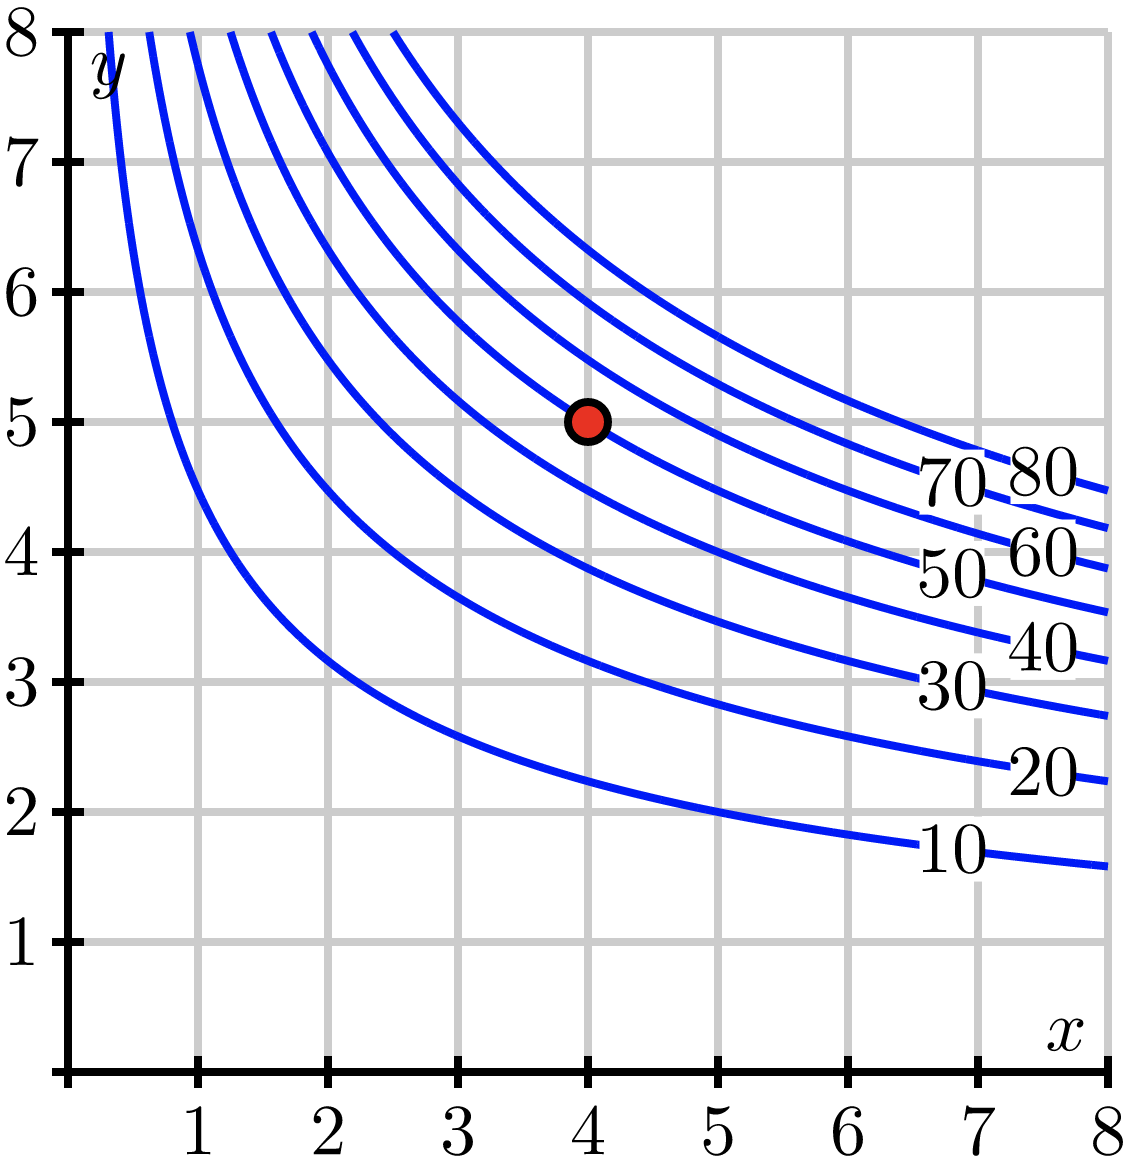
\includegraphics[width=0.5\textwidth]{2-2-14.png}
        \end{center}
        
        \begin{red}
            To find $f_x(4,5)$: I'm going to stand at the point $(4,5)$ and, holding $y$ constant, take a small step in the $x$ direction, and see what happens to my output values.
            
            When I'm on the point $(4,5)$, I'm on the $z = 50$ contour, so I know that $f(4,5) = 50$. If I take a little step in the $x$ direction, I land just a little above the $z = 60$ contour, so I know that $f(4+1, 5) \approx 60$ or $62$ish. Therefore, my step of 1 kg has produced a change of 10 or 12 Joules, so $f_x(4,5) \approx 10/1$ or $12/1$ Joules per kg. This is pretty close to the value we calculated earlier, $\tfrac{25}{2} = 12.5$.
            
            To find $f_y(4,5)$: I'm going to stand at the point $(4,5)$ and, holding $x$ constant, take a small step in the $y$ direction, and see what happens to my output values.
            
            When I'm on the point $(4,5)$, I'm on the $z = 50$ contour, so I know that $f(4,5) = 50$. If I take a little step in the $y$ direction, I land just a little above the $z = 70$ contour, so I know that $f(4, 5+1) \approx 70$ or $72$ish. Therefore, my step of 1 m/s has produced a change of 20 or 22 Joules, so $f_y(4,5) \approx 20/1$ or $22/1$ Joules per m/s. This is pretty close to the value we calculated earlier, $20$.
            
            
        \end{red}
    \end{enumerate}

\end{enumerate}

\begin{red}
\textbf{Learning Targets Reflection:} Maybe S1, maybe S2, D5, D6.
\end{red}

\end{document}